\begin{figure}
\begin{center}

\begin{subfigure}{\textwidth}
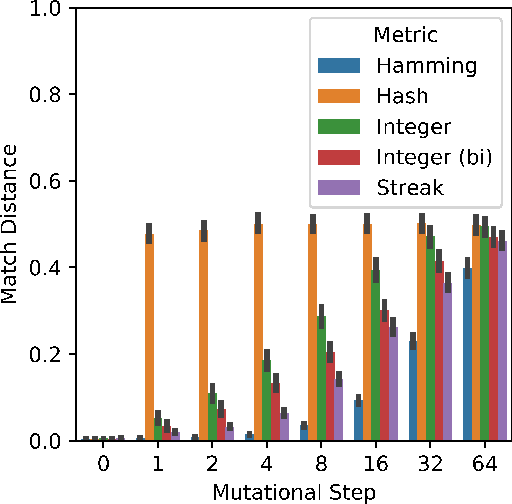
\includegraphics[width=\textwidth]{img/mutational_walk_sampled_start_64/bitweight=0dot5+seed=1+title=mutational_walk_barplot+_data_hathash_hash=2137b5ab8659c35e+_script_fullcat_hash=982405ca713eba73+ext=}
\caption{
Error bars represent 95\% confidence intervals.
Note logarithmic scale on the $x$ axis.
}
\label{fig:mutational_walk_sampled_start_64_barplot}
\end{subfigure}

\begin{subfigure}{\textwidth}
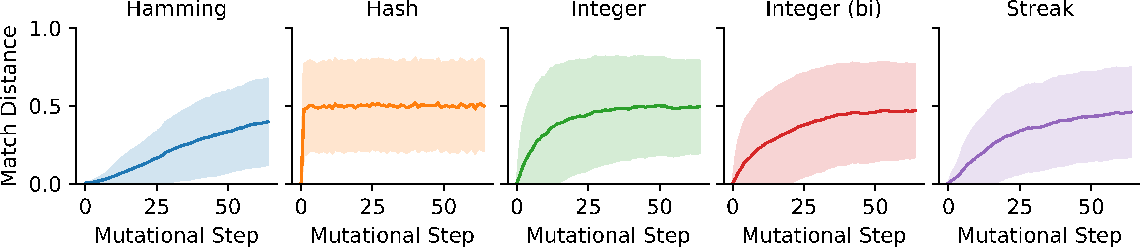
\includegraphics[width=\textwidth]{img/mutational_walk_sampled_start_64/bitweight=0dot5+seed=1+title=mutational_walk_lineplot+_data_hathash_hash=2137b5ab8659c35e+_script_fullcat_hash=982405ca713eba73+ext=}
\caption{
Alternate visualization, shaded area represents standard deviation.
}
\end{subfigure}

\caption{
Match distance along mutational walks from 64-bit tags sampled for initial match distance $<0.01$.
}
\label{fig:mutational_walk_sampled_start}

\end{center}
\end{figure}
